%SOP Template 
% Version 02 Added revision date
% Version 03 Added TOC and acknowledgements
%           New SOP3_alpha.cls


\documentclass[12pt]{../SOP4_alpha}\usepackage[]{graphicx}\usepackage[]{xcolor}
% maxwidth is the original width if it is less than linewidth
% otherwise use linewidth (to make sure the graphics do not exceed the margin)
\makeatletter
\def\maxwidth{ %
  \ifdim\Gin@nat@width>\linewidth
    \linewidth
  \else
    \Gin@nat@width
  \fi
}
\makeatother

\definecolor{fgcolor}{rgb}{0.345, 0.345, 0.345}
\newcommand{\hlnum}[1]{\textcolor[rgb]{0.686,0.059,0.569}{#1}}%
\newcommand{\hlstr}[1]{\textcolor[rgb]{0.192,0.494,0.8}{#1}}%
\newcommand{\hlcom}[1]{\textcolor[rgb]{0.678,0.584,0.686}{\textit{#1}}}%
\newcommand{\hlopt}[1]{\textcolor[rgb]{0,0,0}{#1}}%
\newcommand{\hlstd}[1]{\textcolor[rgb]{0.345,0.345,0.345}{#1}}%
\newcommand{\hlkwa}[1]{\textcolor[rgb]{0.161,0.373,0.58}{\textbf{#1}}}%
\newcommand{\hlkwb}[1]{\textcolor[rgb]{0.69,0.353,0.396}{#1}}%
\newcommand{\hlkwc}[1]{\textcolor[rgb]{0.333,0.667,0.333}{#1}}%
\newcommand{\hlkwd}[1]{\textcolor[rgb]{0.737,0.353,0.396}{\textbf{#1}}}%
\let\hlipl\hlkwb

\usepackage{framed}
\makeatletter
\newenvironment{kframe}{%
 \def\at@end@of@kframe{}%
 \ifinner\ifhmode%
  \def\at@end@of@kframe{\end{minipage}}%
  \begin{minipage}{\columnwidth}%
 \fi\fi%
 \def\FrameCommand##1{\hskip\@totalleftmargin \hskip-\fboxsep
 \colorbox{shadecolor}{##1}\hskip-\fboxsep
     % There is no \\@totalrightmargin, so:
     \hskip-\linewidth \hskip-\@totalleftmargin \hskip\columnwidth}%
 \MakeFramed {\advance\hsize-\width
   \@totalleftmargin\z@ \linewidth\hsize
   \@setminipage}}%
 {\par\unskip\endMakeFramed%
 \at@end@of@kframe}
\makeatother

\definecolor{shadecolor}{rgb}{.97, .97, .97}
\definecolor{messagecolor}{rgb}{0, 0, 0}
\definecolor{warningcolor}{rgb}{1, 0, 1}
\definecolor{errorcolor}{rgb}{1, 0, 0}
\newenvironment{knitrout}{}{} % an empty environment to be redefined in TeX

\usepackage{alltt}

\usepackage[english]{babel}


\title{Hach DR3900}
\date{X/XX/XXXX}
\author{Reseacher Name}
\approved{TBD}
\ReviseDate{\today}
\SOPno{X}
\IfFileExists{upquote.sty}{\usepackage{upquote}}{}
\begin{document}


\maketitle

\section{Scope and Application}

\NP The scope of this SOP is train researchers...

\NP The applications of this SOP are for...

\section{Summary of Method}

\NP This SOP does this...

\tableofcontents

\newpage

\section{Acknowledgements}

\section{Definitions}

\NP Term1: is...

\section{Biases and Interferences}

\NP Biases and interferences can come from...

\section{Health and Safety}

\NP Describe the risk...


\subsection{Safety and Personnnel Protective Equipment}


\section{Personnel \& Training Responsibilities}

\NP Researchers training is required before this the procedures in this method can be used... 

\NP Researchers using this SOP should be trained for the following SOPs:

\begin{itemize}
  \item SOP01 Laboratory Safety
  \item SOP02 Field Safety
\end{itemize}

\section{Required Materials and Apparati}

\NP Item 1 w/catalog number!

\NP Item 2

\section{Reagents and Standards}

\section{Estimated Time}

\NP This procedure requires XX minutes...

\section{Sample Collection, Preservation, and Storage}
\section{Procedure}
\subsection {How to do a measurement}
\NP Select the applicable program from the programs menu (e.g., Stored Programs, User Programs, Favorites).
\NP Install the cell adapter, if necessary.
\NP Push Start to start the program
\NP Prepare the blank according to the method document. Close the sample cell and clean the optical faces of the sample cell with a lint- free cloth.
\NP Insert the blank sample cell into the cell compartment. Make sure to install the blank sample cell in the correct and in a consistent orientation so that the results are more repeatable and precise. Refer to figure 1.
\begin{figure}
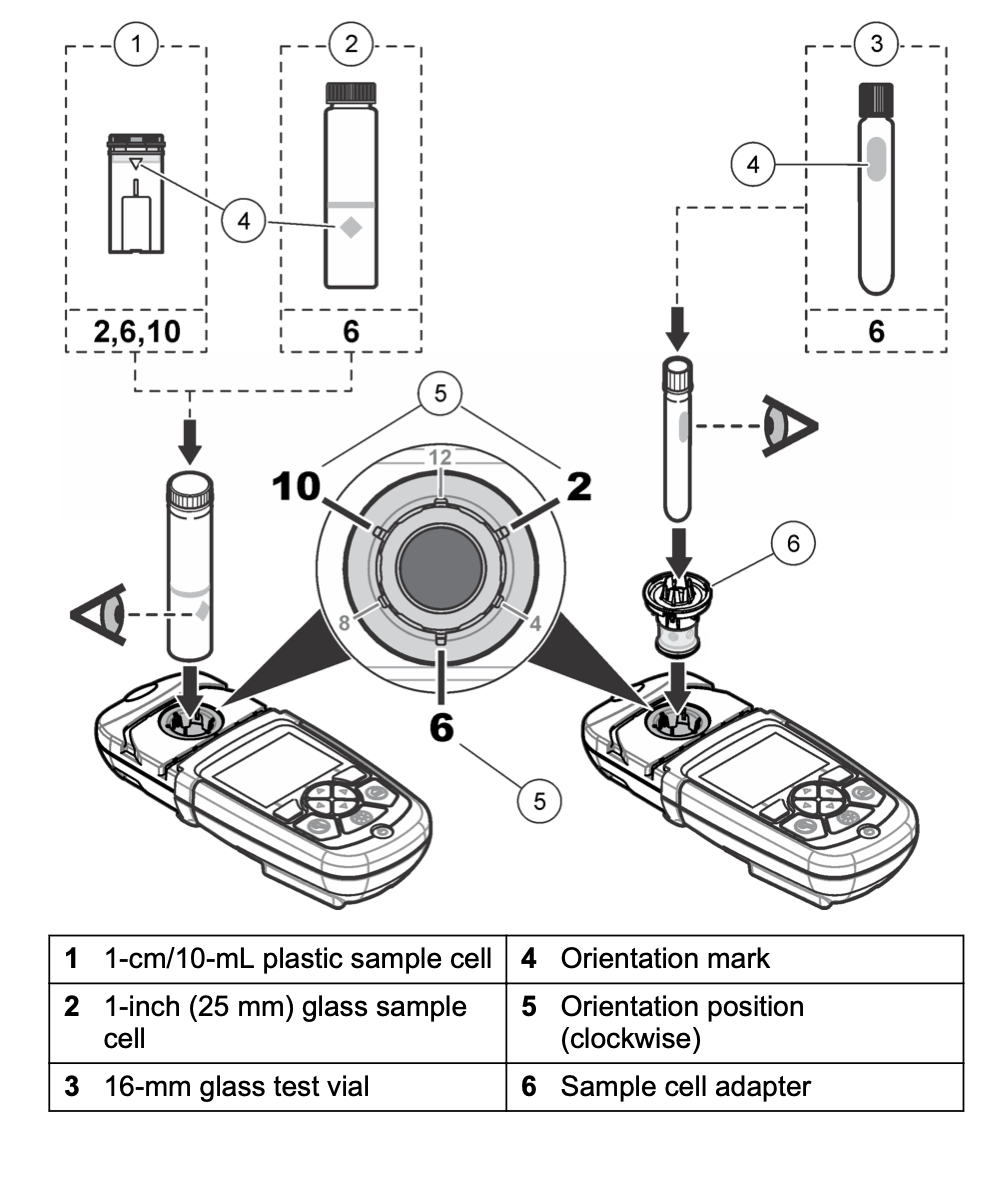
\includegraphics{Graphics/Samplecell.png}
\end{figure}
\NP Close the instrument cap to prevent light interferences
\NP Push Zero. The display shows a concentration of zero (e.g., mg/L, ABS, μg/L).
\NP Prepare the sample. Add reagents as specified by the method document.
\NP Select Options>Start Timer to use the stored timers within the program.
\NP Close the sample cell and clean the optical surfaces of the cell with a lint-free cloth
\NP Insert the sample into the cell compartment. Make sure to install the sample cell in the correct and in a consistent orientation so that the results are more repeatable and precise. 
\NP Close the instrument cap to prevent light interferences.
\NP Push Read. The display shows the results in the selected units.

\section{Data Analysis and Calculations}

\section{QC/QA Criteria}

\section{Trouble Shooting}

\section{References}

\NP APHA, AWWA. WEF. (2012) Standard Methods for examination of water and wastewater. 22nd American Public Health Association (Eds.). Washington. 1360 pp. (2014).

\end{document}
